\chapter{Variabili atomiche in Java}
Nel package \verb#java.util.concurrent.atomic# sono definite una serie di classi che supportano le operazioni atomiche su singole variabili.
\\In ambienti multi-threaded, dove diversi thread operano su una singola variabile, un thread per volta può accedere e leggere o modificare la variabile. Se così non fosse si creerebbero stati di inconsistenza dei dati (race condition).
\\Tipi di atomicità:
\begin{description}
    \item[Reale:] una sola istruzione di CPU viene impiegata per eseguire l'operazione
    \item[Virtuale:] il thread “crede” di avere accesso atomico alla variabile, concettualmente simile a monitor (oggetti con metodi synchronized)
\end{description}

\section{Il problema della visibilità}
Per le applicazioni multi-thread, è necessario garantire due condizioni per un comportamento coerente:
\begin{description}
    \item[Mutua esclusione:] solo un thread esegue una sezione critica alla volta.
    \item[Visibilità:] le modifiche apportate da un thread ai dati condivisi sono visibili agli altri thread per mantenere la coerenza dei dati.
\end{description}
Problemi di visibilità si creano quando due thread sono in esecuzione su core diversi, perché le variabili condivise vengono tenute in cache per ragioni di performance.
\\I metodi e i blocchi sincronizzati forniscono entrambe le proprietà, a scapito delle performance.
\\Si può ovviare al problema della visibilità utilizzando variabili \verb#volatile#.
\begin{center}
    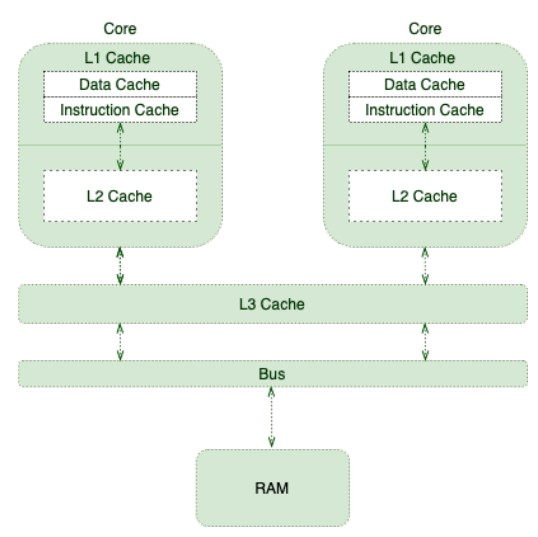
\includegraphics[width=0.675\textwidth]{img/concorrenza177.jpg}
\end{center}

\subsubsection{Esempio: Contatore Non Sincronizzato}
4 slides

\subsection{java.util.concurrent}
Alcune classi della libreria java.util.concurrent hanno delle performance superiori alle loro alternative bloccanti (es. BlockingQueue vs
ConcurrentLinkedQueue), perché?
\begin{itemize}
    \item Variabili atomiche (AtomicInteger, AtomicLong, ecc)
    \item Algoritmi non bloccanti
\end{itemize}
Variabili atomiche: java.util.concurrent.atomic
\begin{itemize}
    \item "Variabili volatile migliorate"
    \item Operazioni di aggiornamento che non richiedono lock, sono basate su operazioni atomiche
\end{itemize}
Algoritmi non bloccanti
\begin{itemize}
    \item Sono thread-safe senza ricorrere a lock
    \item Usati per process scheduling, garbage collection, implementazione dei lock
    \item Più complessi degli equivalenti basati su lock bloccanti
\end{itemize}

\section{Meccanismo di Locking}
\subsubsection{Lock in breve}
\begin{description}
    \item[1. Acquisizione -] accesso ai diritti di sincronizzazione
    \item[2. Algoritmo di attesa -] spin o sleep in attesa che la sincronizzazione sia disponibile
    \item[3. Rilascio -] i diritti di accesso vengono rilasciati ed altri thread possono richiederli
\end{description}

\subsection{Problemi associati}
Se un thread non riesce ad acquisire un lock viene sospeso.
\\Context switch, risvegliare un thread presenta un costo.
\\Un thread in attesa non può eseguire nessuna operazione.
\\Un thread a bassa priorità può bloccare thread che ne hanno una più alta (priority inversion), infatti quando un thread acquisisce un lock nessun altro thread che ha bisogno di quel lock può proseguire.
\\Il processo di locking viene detto pessimistico. Infatti se la contesa è non è frequente, nella maggior parte dei casi la richiesta e l'esecuzione di un lock non è necessaria ed aggiunge overhead. 

\subsection{Alternative al Locking: optimistic retrying}
Optimistic retrying
\begin{itemize}
    \item Nessuna sincronizzazione in lettura
    \item Per eseguire una scrittura
    \\1. Lettura della variabile (creazione di una copia locale)
    \\2. Aggiornamento della copia
    \\3. Scrittura della variabile se non c'è collisione, altrimenti riprovare
\end{itemize}
Quest'approccio è particolarmente adatto all'aggiornamento delle strutture accessibili per mezzo di un unico indirizzo; es: aggiornamento di un Integer.
\\I processori moderni offrono istruzioni (per la collision detection) di supporto alla tecnica di optimistic retrying.
1: tmp = readMem(pos);
2: tmp = update(tmp)
3: if Collision(pos) goto 1
3: else writeMem(pos,tmp)

\subsection{Strumento: Compare-and-Swap (CAS)}
È una operazione atomica messa a disposizione da alcuni processori che prende in ingresso 3 argomenti:
\begin{itemize}
    \item Una posizione di memoria V
    \item Un valore atteso E
    \item Un nuovo valore N
\end{itemize}
L'aggiornamento ha avuto successo
\begin{itemize}
    \item Se il valore restituito è uguale al valore atteso E
    \item Altrimenti non c'è stato aggiornamento
\end{itemize}
compare-and-set
Come CAS ma restituisce un true se
l'operazione si è conclusa con successo, false
altrimenti







